\documentclass[nooutcomes]{ximera}

\input{../preamble.tex}
\author{Kenneth Berglund}
\license{Creative Commons Attribution-ShareAlike 4.0 International License}
\acknowledgement{https://www.stitz-zeager.com/szca07042013.pdf}

\title{Famous Formulas}

%This is so the pictures show up
\pgfplotsset{compat=1.5.1}

%This is also for pictures
\usetikzlibrary{calc}

%This makes hyperbolas. I found it at https://newbedev.com/can-one-draw-a-hyperbola-with-arguments-in-tikz
%
% #1 optional parameters for \draw
% #2 angle of rotation in degrees
% #3 offset of center as (pointx, pointy) or (name-o-coordinate)
% #4 length of plus (semi)axis, that is axis which hyperbola crosses
% #5 length of minus (semi)axis
% #6 how much of hyperbola to draw in degrees, with 90 you’d reach infinity
%
\newcommand\tikzhyperbola[6][thick]{%
    \draw [#1, rotate around={#2: (0, 0)}, shift=#3]
        plot [variable = \t, samples=1000, domain=-#6:#6] ({#4 / cos( \t )}, {#5 * tan( \t )});
    \draw [#1, rotate around={#2: (0, 0)}, shift=#3]
        plot [variable = \t, samples=1000, domain=-#6:#6] ({-#4 / cos( \t )}, {#5 * tan( \t )});
}

\begin{document}
\begin{abstract}
  
\end{abstract}
\licenseSZ
\maketitle

%\typeout{************************************************}
%\typeout{Introduction}
%\typeout{************************************************}
\section{Introduction}
As a review, we go over the list of famous functions from earlier. Then, we move to a discussion of conic sections. 



%\typeout{************************************************}
%\typeout{Linear Functions}
%\typeout{************************************************}

\section{Linear Functions}
Recall that the graph of a linear function is a line. 

\begin{example}
A prototypical example of a linear function is $$ \mbox{\huge $y=x.$}$$ 

\begin{image}
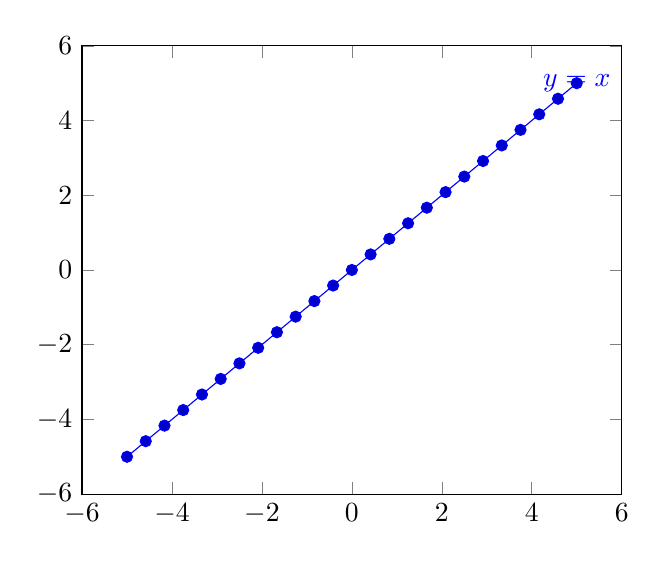
\begin{tikzpicture}
    \begin{axis}
        \addplot{x} node{$y=x$};
    \end{axis}
\end{tikzpicture}
\end{image}

\begin{center}
\(
\begin{array}{ |c || c|  }
 \hline
 \multicolumn{2}{|c|}{\text{\normalfont Important Values of } y=x} \\
\hline
 \hline
 x & y\\
 \hline
 -2&-2\\
 -1&-1\\
 0&0\\
 1&1\\
 2&2\\
 \hline
\end{array}
\)
\end{center}
\end{example}

In general, linear functions can be written as $y=mx+b$ where $m$ and $b$ can be any numbers. We learned that $m$ represents the slope, and $b$ is the $y$-coordinate of the $y$-intercept. You can play with changing the values of $m$ and $b$ on the graph using Desmos and see how that changes the line.  

\begin{center}  
\desmos{japnhapzvn}{800}{600}  
\end{center}

\begin{center}
$
\begin{array}{|l|l|}
 \hline
 \multicolumn{2}{|c|}{\text{\normalfont Properties of Linear Functions } y=mx + b} \\
\hline
 \hline
\text{Periodic?} & \text{If } m = 0 \\ \hline
\text{Odd?} & \text{If } b = 0 \\ \hline
\text{Even?} & \text{If } m = 0 \\ \hline
\text{One-to-one/invertible?} & \text{Yes}\\ \hline
\end{array}
$
\end{center}

\begin{center}
$
\begin{array}{|l|l|}
 \hline
 \multicolumn{2}{|c|}{\text{\normalfont Domain and Range of Linear Functions } y=mx + b} \\
\hline
 \hline
\text{Domain} & (-\infty, \infty) \\ \hline
\text{Range} & \text{If } m \ne 0\text{, } (-\infty, \infty)\text{; if } m = 0 \text{, } \{b\}\\ \hline
\end{array}
$
\end{center}

\newpage

%\typeout{************************************************}
%\typeout{Quadratic Functions}
%\typeout{************************************************}

\section{Quadratic Functions}

Recall that the graph of a quadratic function is a parabola.

\begin{example}
A prototypical example of a quadratic function is $$ \mbox{\huge $y=x^2.$}$$

\begin{image}
\begin{tikzpicture}
    \begin{axis}
        \addplot[smooth]{x^2} node{$y=x^2$};
    \end{axis}
\end{tikzpicture}
\end{image}

\begin{center}
\(
\begin{array}{ |c || c|  }
 \hline
 \multicolumn{2}{|c|}{\text{\normalfont Important Values of } y=x^2} \\
\hline
 \hline
 x & y\\
 \hline
 -2&4\\
 -1&1\\
 0&0\\
 1&1\\
 2&4\\
 \hline
\end{array}
\)
\end{center}
\end{example}

In general, quadratic functions can be written as $y=ax^2+bx+c$ where $a$, $b$, and $c$ can be any numbers.  You can play with changing the values of $a$, $b$, and $c$ on the graph using Desmos and see how that changes the parabola.  

\begin{center}  
\desmos{nmlghfrws9}{800}{600}  
\end{center}

\begin{center}
$
\begin{array}{|l|l|}
 \hline
 \multicolumn{2}{|c|}{\text{\normalfont Properties of Quadratic Functions } y=ax^2 + bx + c, a \ne 0} \\
\hline
 \hline
\text{Periodic?} & \text{No} \\ \hline
\text{Odd?} & \text{No} \\ \hline
\text{Even?} & \text{If } b = 0 \\ \hline
\text{One-to-one/invertible?} & \text{No}\\ \hline
\end{array}
$
\end{center}

\begin{center}
$
\begin{array}{|l|l|}
 \hline
 \multicolumn{2}{|c|}{\text{\normalfont Domain and Range of Quadratic Functions } y=d(x - h)^2 + k} \\
\hline
 \hline
\text{Domain} & (-\infty, \infty) \\ \hline
\text{Range} & \text{If } d > 0\text{, }[k, \infty)\text{; if }d < 0\text{, }(\infty, k]\\ \hline
\end{array}
$
\end{center}

\newpage

%\typeout{************************************************}
%\typeout{Absolute Value}
%\typeout{************************************************}

\section{Absolute Value}
Another important type of function is the absolute value function.  This is the function that takes all $y$-values and makes them positive.  The absolute value function is written as 

$$ \mbox{\huge $y=|x|.$}$$ 

\begin{image}
\begin{tikzpicture}
    \begin{axis}
        \addplot[smooth]{abs(x)} node{$y=|x|$};
    \end{axis}
\end{tikzpicture}
\end{image}

\begin{center}
\(
\begin{array}{ |c || c|  }
 \hline
 \multicolumn{2}{|c|}{\text{\normalfont Important Values of } y=|x|} \\
\hline
 \hline
 x & y\\
 \hline
 -2&2\\ 
-1&1\\ 
0&0\\
 1&1\\
 2&2\\
 \hline
\end{array}
\)
\end{center}

\begin{center}
$
\begin{array}{|l|l|}
 \hline
 \multicolumn{2}{|c|}{\text{\normalfont Properties of the Absolute Value Function } y=|x|} \\
\hline
 \hline
\text{Periodic?} & \text{No} \\ \hline
\text{Odd?} & \text{No} \\ \hline
\text{Even?} & \text{Yes } \\ \hline
\text{One-to-one/invertible?} & \text{No}\\ \hline
\end{array}
$
\end{center}

\begin{center}
$
\begin{array}{|l|l|}
 \hline
 \multicolumn{2}{|c|}{\text{\normalfont Domain and Range of the Absolute Value Function } y=|x|} \\
\hline
 \hline
\text{Domain} & (-\infty, \infty) \\ \hline
\text{Range} & [0, \infty)\\ \hline
\end{array}
$
\end{center}

\newpage

%\typeout{************************************************}
%\typeout{Square Root}
%\typeout{************************************************}

\section{Square Root}
Another famous function is the square root function, $$ \mbox{\huge $y=\sqrt{x}.$}$$ 

\begin{image}
\begin{tikzpicture}
    \begin{axis}
        \addplot[samples=200,domain=0:30]{sqrt(x)};
    \end{axis}
\end{tikzpicture}
\end{image}


\begin{center}
\(
\begin{array}{ |c || c|  }
 \hline
 \multicolumn{2}{|c|}{\text{\normalfont Important Values of } y=\sqrt{x}} \\
\hline
 \hline
 x & y\\
 \hline
 0&0\\
 1&1\\
 4&2\\
 9&3\\
 25&5\\
 \hline
\end{array}
\)
\end{center}

\begin{center}
$
\begin{array}{|l|l|}
 \hline
 \multicolumn{2}{|c|}{\text{\normalfont Properties of the Square Root Function } y=\sqrt{x}} \\
\hline
 \hline
\text{Periodic?} & \text{No} \\ \hline
\text{Odd?} & \text{No} \\ \hline
\text{Even?} & \text{No} \\ \hline
\text{One-to-one/invertible?} & \text{Yes}\\ \hline
\end{array}
$
\end{center}

\begin{center}
$
\begin{array}{|l|l|}
 \hline
 \multicolumn{2}{|c|}{\text{\normalfont Domain and Range of the Square Root Function } y=\sqrt{x}} \\
\hline
 \hline
\text{Domain} & [0, \infty) \\ \hline
\text{Range} & [0, \infty) \\ \hline
\end{array}
$
\end{center}
\newpage

%\typeout{************************************************}
%\typeout{Exponential}
%\typeout{************************************************}

\section{Exponential}
Another famous function is the exponential growth function, $$ \mbox{\huge $y=e^{x}.$}$$ 

Here $e$ is the mathematical constant known as Euler's number.  $e \approx 2.71828 .$.

\begin{image}
\begin{tikzpicture}
    \begin{axis}
        \addplot[samples=200,domain=-10:4]{e^x};
    \end{axis}
\end{tikzpicture}
\end{image}

\begin{center}
\(
\begin{array}{ |c || c|  }
 \hline
 \multicolumn{2}{|c|}{\text{\normalfont Important Values of } y=e^x} \\
\hline
 \hline
 x & y\\
 \hline
 0&1\\[2ex]
 1&e\\[2ex]
 -1&\frac{1}{e}\\[2ex]
 \hline
\end{array}
\)
\end{center}

In general, we can talk about exponential functions of the form $y=b^{x}$ where $b$ is a positive number not equal to $1$.  You can play with changing the values of $b$ on the graph using Desmos and see how that changes the graph.  Pay particular attention to the difference between $b>1$ and $0<b<1$.

\begin{center}  
%\desmos{dgcwh0chfv}{800}{600}  
\desmos{qsmvb7tiex}{800}{600}
\end{center}

\begin{center}
$
\begin{array}{|l|l|}
 \hline
 \multicolumn{2}{|c|}{\text{\normalfont Properties of the Exponential Functions } y=b^x} \\
\hline
 \hline
\text{Periodic?} & \text{No} \\ \hline
\text{Odd?} & \text{No} \\ \hline
\text{Even?} & \text{No} \\ \hline
\text{One-to-one/invertible?} & \text{Yes} \\ \hline
\end{array}
$
\end{center}

\begin{center}
$
\begin{array}{|l|l|}
 \hline
 \multicolumn{2}{|c|}{\text{\normalfont Domain and Range of the Exponential Functions } y=b^x} \\
\hline
 \hline
\text{Domain} & (-\infty, \infty) \\ \hline
\text{Range} & [0, \infty) \\ \hline
\end{array}
$
\end{center}


\newpage

%\typeout{************************************************}
%\typeout{Logarithms}
%\typeout{************************************************}

\section{Logarithm}
Another group of famous functions are logarithms.

\begin{example}
The most famous logarithm function is
 $$ \mbox{\huge $y=\ln(x)=\log_{e}(x)$.}$$ 
Here $e$ is the mathematical constant known as Euler's number. $e \approx 2.71828$.

\begin{image}
\begin{tikzpicture}
    \begin{axis}
        \addplot[samples=200,domain=0.01:8]{ln(x)};
    \end{axis}
\end{tikzpicture}
\end{image}

\begin{center}
\(
\begin{array}{ |c || c|  }
 \hline
 \multicolumn{2}{|c|}{\text{\normalfont Important Values of } y=ln(x)} \\
\hline
 \hline
 x & y\\
 \hline
0&\text{\normalfont undefined}\\ 
\frac{1}{e}&-1\\ [2ex]
1&0\\[2ex]
 e&1\\[2ex]
 \hline
\end{array}
\)
\end{center}

\end{example}

You may notice that the table of values for $y=\ln(x)$ and $y=e^x$ are similiar.  This is becase these two functions are interconnected.  We will explore this more later in the course.

In general, we can talk about logarithmic functions of the form $y=\log_b(x)$ where $b$ is a positive number not equal to $1$.  You can play with changing the values of $b$ on the graph using Desmos and see how that changes the graph.  Pay particular attention to the difference between $b>1$ and $0<b<1$.

\begin{center}  
\desmos{lxllnpdi6w}{800}{600}  
\end{center}

\begin{center}
$
\begin{array}{|l|l|}
 \hline
 \multicolumn{2}{|c|}{\text{\normalfont Properties of the Logarithm Functions } y=\log_b(x)} \\
\hline
 \hline
\text{Periodic?} & \text{No} \\ \hline
\text{Odd?} & \text{No} \\ \hline
\text{Even?} & \text{No} \\ \hline
\text{One-to-one/invertible?} & \text{Yes} \\ \hline
\end{array}
$
\end{center}

\begin{center}
$
\begin{array}{|l|l|}
 \hline
 \multicolumn{2}{|c|}{\text{\normalfont Domain and Range of the Logarithm Functions } y=\log_b(x)} \\
\hline
 \hline
\text{Domain} & [0, \infty) \\ \hline
\text{Range} & (-\infty, \infty) \\ \hline
\end{array}
$
\end{center}

\newpage

%\typeout{************************************************}
%\typeout{Sine}
%\typeout{************************************************}

\section{Sine}
Another important function is the sine function, $$ \mbox{\huge $y=\sin(x)$.}$$ 


This function comes from trigonometry. In the table below we will use another mathematical constant, $\pi$ (``pi" pronounced pie). $\pi \approx 3.14159$.

\begin{image}
\begin{tikzpicture}
    \begin{axis}[ymin=-2, ymax=2,
		   %xtick={-6.28318, -4.7123889, -3.14159, -1.5708, 1.5708, 3.14159, 4.7123889, 6.28318},
    xticklabels={
        $-\frac{3\pi}{2}$, $-\pi$, $\frac{\pi}{2}$, $0$,
        $\frac{\pi}{2}$, $\pi$, $\frac{3\pi}{2}$, $2\pi$
    }, ]
        \addplot[samples=200]{sin(pi/4*deg(x))};
    \end{axis}
\end{tikzpicture}
\end{image}

\begin{center}
\(
\begin{array}{ |c || c|  }
 \hline
 \multicolumn{2}{|c|}{\text{\normalfont Important Values of } y=\sin(x)} \\
\hline
 \hline
 x & y\\
 \hline

 -\pi&0\\

 -\frac{\pi}{2}&-1\\[2ex]

 0&0\\

 \frac{\pi}{2}&1\\[2ex]

 \pi&0\\

\frac{3\pi}{2}&-1\\[2ex]

 2 \pi&0\\
\hline
\end{array}
\)
\end{center}


\begin{center}
$
\begin{array}{|l|l|}
 \hline
 \multicolumn{2}{|c|}{\text{\normalfont Properties of the Sine Function } y=\sin(x)} \\
\hline
 \hline
\text{Periodic?} & \text{Yes, with period }2\pi \\ \hline
\text{Odd?} & \text{Yes} \\ \hline
\text{Even?} & \text{No} \\ \hline
\text{One-to-one/invertible?} & \text{No} \\ \hline
\end{array}
$
\end{center}

\begin{center}
$
\begin{array}{|l|l|}
 \hline
 \multicolumn{2}{|c|}{\text{\normalfont Domain and Range of the Sine Function } y= \sin(x)} \\
\hline
 \hline
\text{Domain} & (-\infty, \infty) \\ \hline
\text{Range} & [-1, 1] \\ \hline
\end{array}
$
\end{center}

In general, we can consider $y=a\sin(bx)$.  You can play with changing the values of $a$ and $b$ on the graph using Desmos and see how that changes the graph.  

\begin{center}  
\desmos{vkxzcfv2aq}{800}{600}  
\end{center}



\newpage

%\typeout{************************************************}
%\typeout{Cosine}
%\typeout{************************************************}

\section{Cosine}
A function introduced in Section 3-2 is the cosine function, $$ \mbox{\huge $y=\cos(x)$.}$$ 


As with sine, the cosine function comes from trigonometry. In the table below we will again use $\pi$.

\begin{image}
\begin{tikzpicture}
    \begin{axis}[ymin=-2, ymax=2,
		   %xtick={-6.28318, -4.7123889, -3.14159, -1.5708, 1.5708, 3.14159, 4.7123889, 6.28318},
    xticklabels={
        $-\frac{3\pi}{2}$, $-\pi$, $\frac{\pi}{2}$, $0$,
        $\frac{\pi}{2}$, $\pi$, $\frac{3\pi}{2}$, $2\pi$
    }, ]
        \addplot[samples=200]{cos(pi/4*deg(x))};
    \end{axis}
\end{tikzpicture}
\end{image}

\begin{center}
\(
\begin{array}{ |c || c|  }
 \hline
 \multicolumn{2}{|c|}{\text{\normalfont Important Values of } y=\cos(x)} \\
\hline
 \hline
 x & y\\
 \hline

 -\pi&-1\\

 -\frac{\pi}{2}&0\\[2ex]

 0&1\\

 \frac{\pi}{2}&0\\[2ex]

 \pi&-1\\

\frac{3\pi}{2}&0\\[2ex]

 2 \pi&1\\
\hline
\end{array}
\)
\end{center} 


\begin{center}
$
\begin{array}{|l|l|}
 \hline
 \multicolumn{2}{|c|}{\text{\normalfont Properties of the Cosine Function } y=\cos(x)} \\
\hline
 \hline
\text{Periodic?} & \text{Yes, with period }2\pi \\ \hline
\text{Odd?} & \text{No} \\ \hline
\text{Even?} & \text{Yes} \\ \hline
\text{One-to-one/invertible?} & \text{No} \\ \hline
\end{array}
$
\end{center}


\begin{center}
$
\begin{array}{|l|l|}
 \hline
 \multicolumn{2}{|c|}{\text{\normalfont Domain and Range of the Cosine Function } y=\cos(x)} \\
\hline
 \hline
\text{Domain} & (-\infty, \infty) \\ \hline
\text{Range} & [-1, 1] \\ \hline
\end{array}
$
\end{center}

In general, we can consider $y=a\cos(bx)$.  You can play with changing the values of $a$ and $b$ on the graph using Desmos and see how that changes the graph.  

\begin{center}  
\desmos{kvmz1kt19n}{800}{600}  
\end{center}

\newpage

%\typeout{************************************************}
%\typeout{Tangent}
%\typeout{************************************************}

\section{Tangent}
A function introduced in Section 4-1 is the tangent function, $$ \mbox{\huge $y=\tan(x)$.}$$ 

	\begin{image}
		\begin{tikzpicture}
			\begin{axis}[
		            xmin=-6.75,xmax=6.75,ymin=-5.5,ymax=5.5,
		            axis lines=center,
		            xtick={-6.28, -4.71, -3.14, -1.57, 0, 1.57, 3.142, 4.71, 6.28},
		            xticklabels={$-2\pi$,$-3\pi/2$,$-\pi$, $-\pi/2$, $0$, $\pi/2$, $\pi$, $3\pi/2$, $2\pi$},
		            ytick={-5,...,5},
		            minor ytick=,minor xtick=,
		            width=0.75\linewidth,
		            height=0.75\linewidth,
		            xlabel=$x$, ylabel=$x$,
%			    clip=false,
			    grid style={dashed, gray!40}
		          ]        
		          \addplot [very thick, penColor, samples=100,smooth, domain=(-1.56:1.56)] {tan(deg(x))};% node [pos=0.51, penColor2, right] {$t(x)$};
		          \addplot [very thick, penColor, samples=100,smooth, domain=(1.58:4.7)] {tan(deg(x))};
		          \addplot [very thick, penColor, samples=100,smooth, domain=(4.9:6.28)] {tan(deg(x))};
		          \addplot [very thick, penColor, samples=100,smooth, domain=(-4.7:-1.58)] {tan(deg(x))};
		          \addplot [very thick, penColor, samples=100,smooth, domain=(-6.28:-4.9)] {tan(deg(x))};          		          
		        \end{axis}
		\end{tikzpicture}
	\end{image}

\begin{center}
\(
\begin{array}{ |c || c|  }
 \hline
 \multicolumn{2}{|c|}{\text{\normalfont Important Values of } y=\tan(x)} \\
\hline
 \hline
 x & y\\
 \hline

 -\pi&0\\

 -\frac{\pi}{2}& \text{undefined}\\[2ex]

 0&0\\

 \frac{\pi}{2}&\text{undefined}\\[2ex]

 \pi&0\\

\frac{3\pi}{2}&\text{undefined}\\[2ex]

 2 \pi&0\\
\hline
\end{array}
\)
\end{center} 

\begin{center}
$
\begin{array}{|l|l|}
 \hline
 \multicolumn{2}{|c|}{\text{\normalfont Properties of the Tangent Function } y=\tan(x)} \\
\hline
 \hline
\text{Periodic?} & \text{Yes, with period }\pi \\ \hline
\text{Odd?} & \text{Yes} \\ \hline
\text{Even?} & \text{No} \\ \hline
\text{One-to-one/invertible?} & \text{No}\\
\hline
\end{array}
$
\end{center}


\begin{center}
$
\begin{array}{|l|l|}
 \hline
 \multicolumn{2}{|c|}{\text{\normalfont Domain and Range of the Tangent Function } y=\tan(x)} \\
\hline
 \hline
\text{Domain} & \cdots \cup \left(-\frac{5\pi}{2}, -\frac{3\pi}{2}\right) \cup \left(-\frac{3\pi}{2}, -\frac{\pi}{2}\right) \cup \left(\frac{\pi}{2}, \frac{3\pi}{2}\right) \cup \left(\frac{3\pi}{2}, \frac{5\pi}{2}\right) \cup \cdots \\ \hline
\text{Range} & (-\infty, \infty) \\ \hline
\end{array}
$
\end{center}

In general, we can consider $y=a\tan(bx)$.  You can play with changing the values of $a$ and $b$ on the graph using Desmos and see how that changes the graph.  

\begin{center}  
\desmos{1je3xt6hag}{800}{600}  
\end{center}


\end{document}
